\section{Visualizations} \label{app:vis}

We provide additional qualitative results comparing all evaluated methods on all four datasets.

\subsection{Latent Space Visualizations} \label{app:latent_vis}

Figure~\ref{fig:latents_appendix} shows a PCA projection of the task-level latent codes $\mathbf{r}$ produced by the \gls{peach} encoder across all four environments. Each point corresponds to a single test task, colored by its material properties. 
The smooth, structured organization of the latent space, particularly the near-perfect one-dimensional manifold recovered for the single-parameter environments \texttt{Sheet Deformation} and \texttt{Deforming Block}, demonstrates that the encoder successfully disentangles material properties from trajectory-level variation, without any explicit supervision on the latent space geometry.



\begin{figure}[htbp]
    \centering

    \begin{minipage}{0.24\textwidth}
        \centering
        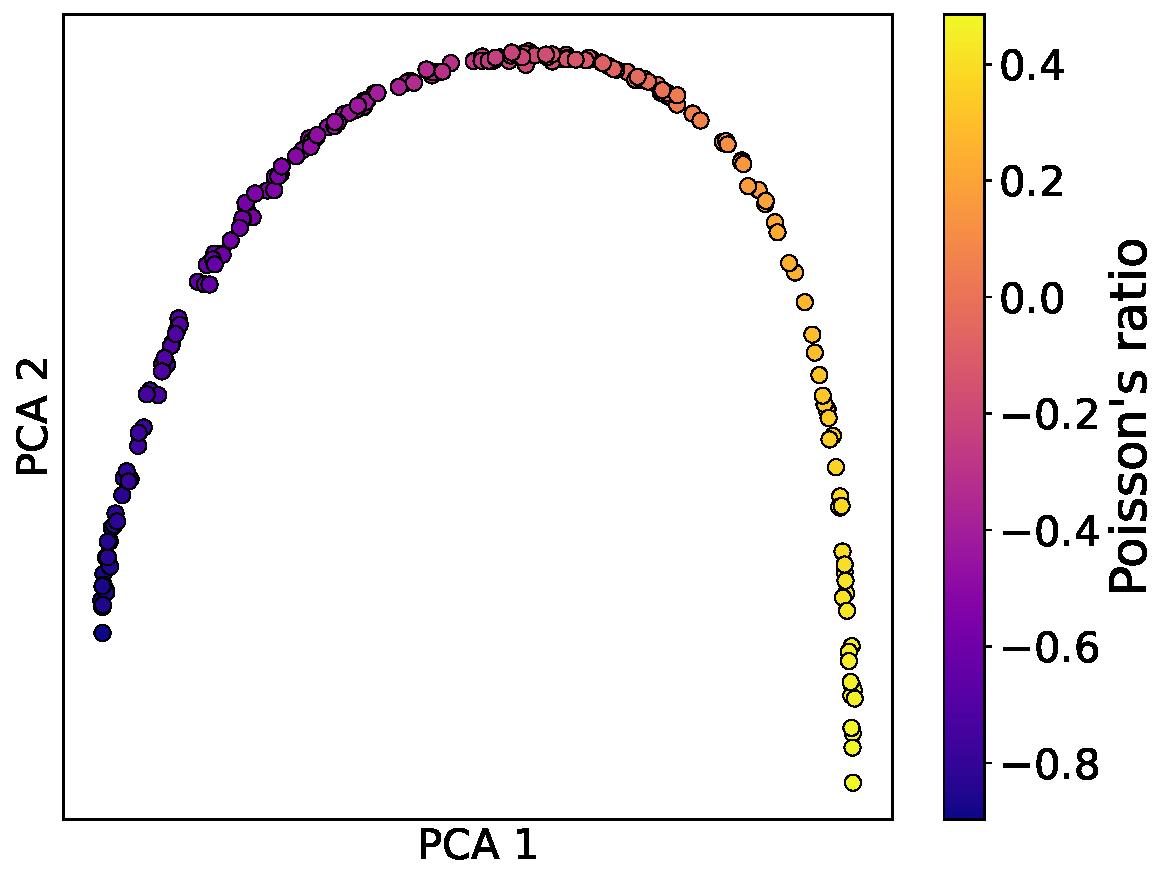
\includegraphics[width=\textwidth]{figures/latent_space_vis/pca_peach_db_poisson.pdf}\\
        {\small \hspace{-1mm}\texttt{Deforming Block}}
    \end{minipage}
    \begin{minipage}{0.24\textwidth}
        \centering
        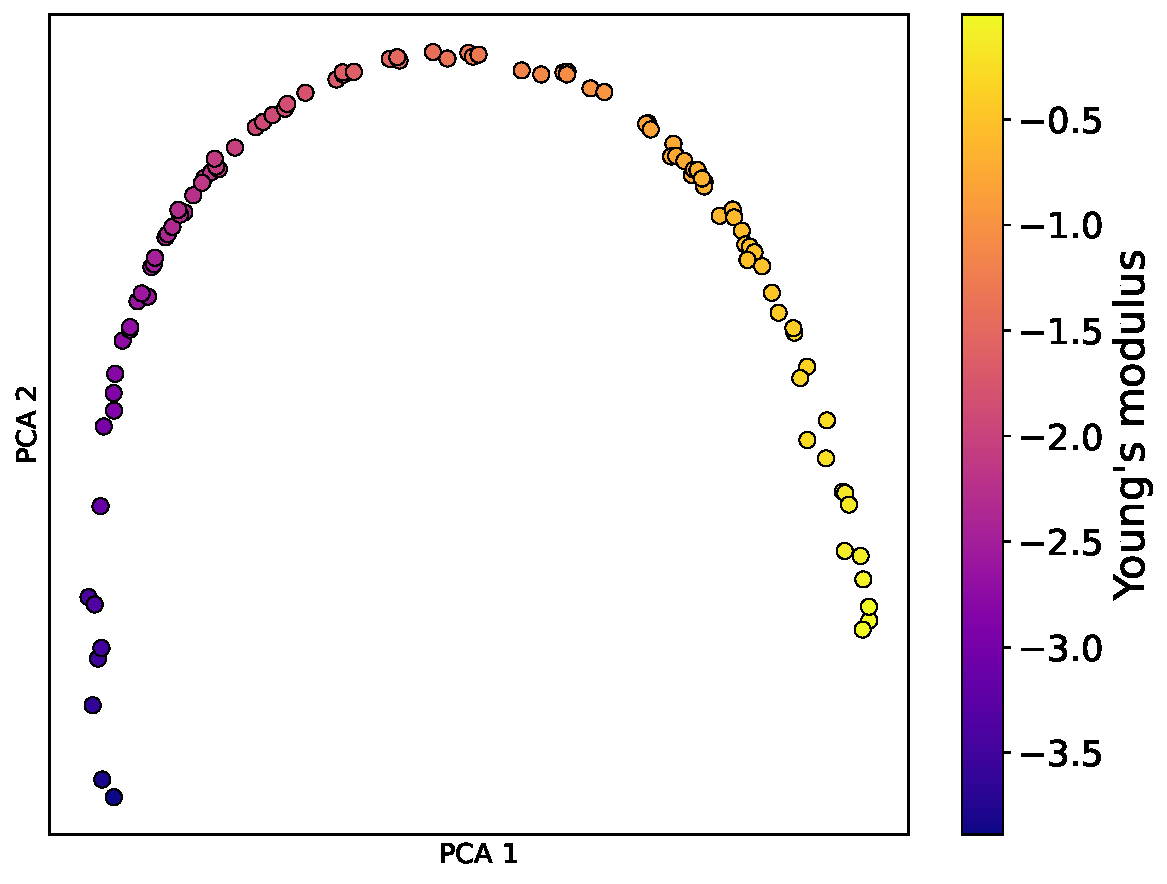
\includegraphics[width=\textwidth]{figures/latent_space_vis/pca_peach_sd_young_modulus.pdf}\\
        {\small \hspace{-2mm}\texttt{Sheet Deformation}}
    \end{minipage}
    \begin{minipage}{0.24\textwidth}
        \centering
        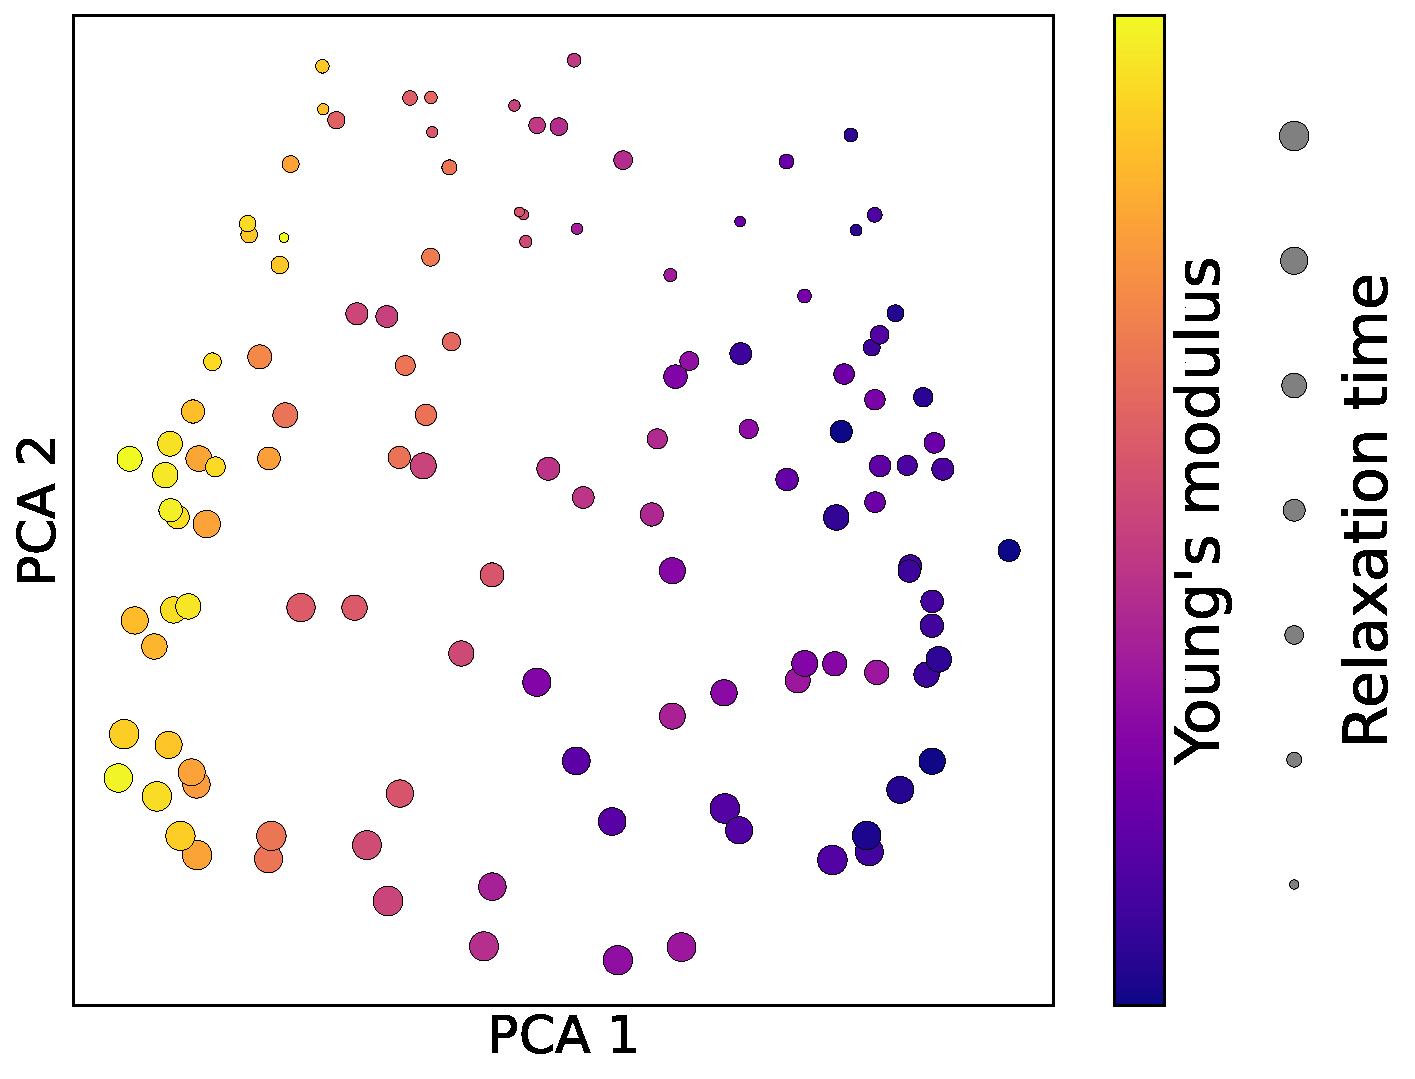
\includegraphics[width=\textwidth]{figures/latent_space_vis/pca_peach_bbv_bivariate.pdf}\\
        {\small \hspace{-1mm}\texttt{Bending Beam}}
    \end{minipage}
    \begin{minipage}{0.24\textwidth}
        \centering
        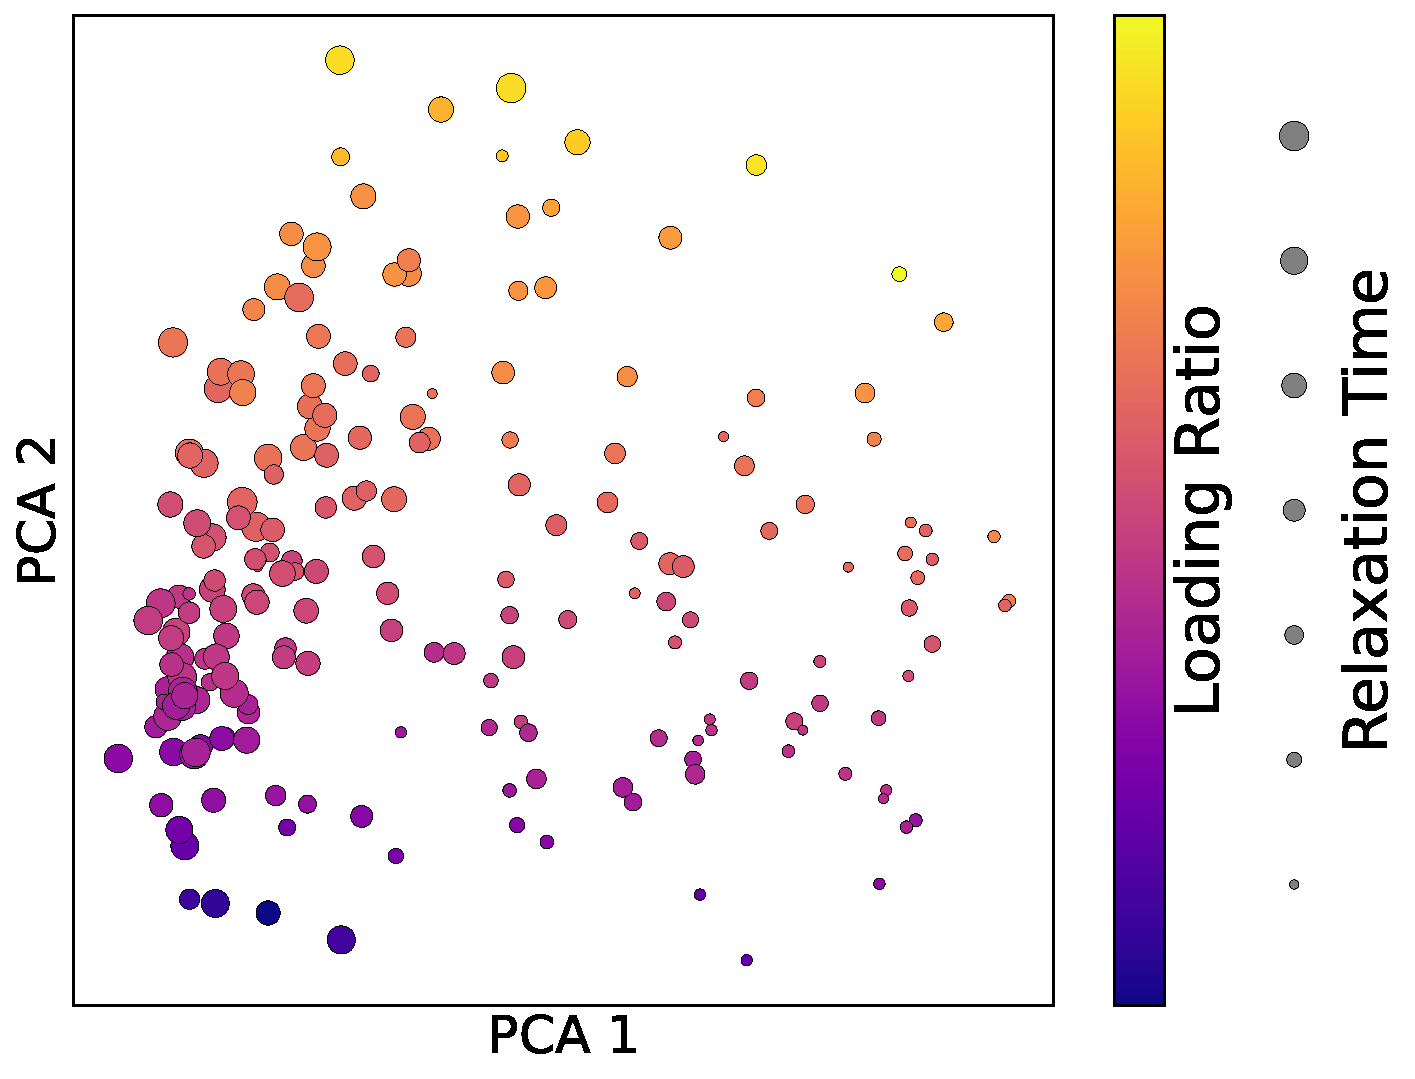
\includegraphics[width=\textwidth]{figures/latent_space_vis/pca_peach_trampoline_bivariate.pdf}\\
        {\small \hspace{-2mm}\texttt{Trampoline}}
    \end{minipage}

    \caption{
        PCA visualization of the latent space on the Deforming block, Sheet deformation, Bending beam and Trampoline environment (left to right).
        Each point represents an encoded task, with different coloring and scaling references based on the task's material properties.
    }
    \label{fig:latents_appendix}
\end{figure}

\subsection{Qualitative Trajectory Predictions}

We provide qualitative trajectory predictions for all evaluated datasets.
Figure~\ref{fig:qualitative_trajectories_db} shows results for the \texttt{Deforming Block} dataset,
Figure~\ref{fig:qualitative_trajectories_sd} for \texttt{Sheet Deformation},
Figure~\ref{fig:qualitative_trajectories_trampoline} for the \texttt{Trampoline} dataset, and
Figure~\ref{fig:qualitative_trajectories_bbv} for \texttt{Bending Beam}.

% =============================================================
%  DEFORMING BLOCK  –  Single figure (all methods)
% =============================================================
\begin{figure*}[p]
    \centering
    {\Large \textbf{Deforming Block}}\\[1em]
    \vfill

    % helper macros (adjust trim once here)
    \newcommand{\rowlabel}[1]{%
        \begin{minipage}[c]{0.05\textwidth}\centering\rotatebox{90}{\scriptsize\textbf{\shortstack{#1}}}\end{minipage}%
    }
    \newcommand{\img}[1]{%
        \includegraphics[width=0.158\textwidth, trim=9cm 2cm 9cm 2cm, clip, valign=m]{#1}%
    }
    \newcommand{\pointcloud}[1]{%
        \includegraphics[width=\textwidth, trim=10cm 4cm 10cm 4cm, clip, valign=m]{#1}%
    }

    % Row 1: PEACH
    \rowlabel{PEACH}%
    \img{figures/qualitative_trajectories_db/PEACH/frame_0000.png}\hspace{-1pt}%
    \img{figures/qualitative_trajectories_db/PEACH/frame_0006.png}\hspace{-1pt}%
    \img{figures/qualitative_trajectories_db/PEACH/frame_0015.png}\hspace{-1pt}%
    \img{figures/qualitative_trajectories_db/PEACH/frame_0021.png}\hspace{-1pt}%
    \img{figures/qualitative_trajectories_db/PEACH/frame_0032.png}\hspace{-1pt}%
    \img{figures/qualitative_trajectories_db/PEACH/frame_0051.png}\\[0.4em]

    % Row 2: No Context
    \rowlabel{No Context}%
    \img{figures/qualitative_trajectories_db/MANGO_Dummy_Dec_No_Context/frame_0000.png}\hspace{-1pt}%
    \img{figures/qualitative_trajectories_db/MANGO_Dummy_Dec_No_Context/frame_0006.png}\hspace{-1pt}%
    \img{figures/qualitative_trajectories_db/MANGO_Dummy_Dec_No_Context/frame_0015.png}\hspace{-1pt}%
    \img{figures/qualitative_trajectories_db/MANGO_Dummy_Dec_No_Context/frame_0021.png}\hspace{-1pt}%
    \img{figures/qualitative_trajectories_db/MANGO_Dummy_Dec_No_Context/frame_0032.png}\hspace{-1pt}%
    \img{figures/qualitative_trajectories_db/MANGO_Dummy_Dec_No_Context/frame_0051.png}\\[0.4em]

    % Row 3: MANGO Decoder
    \rowlabel{MANGO}%
    \img{figures/qualitative_trajectories_db/MANGO_Decoder/frame_0000.png}\hspace{-1pt}%
    \img{figures/qualitative_trajectories_db/MANGO_Decoder/frame_0006.png}\hspace{-1pt}%
    \img{figures/qualitative_trajectories_db/MANGO_Decoder/frame_0015.png}\hspace{-1pt}%
    \img{figures/qualitative_trajectories_db/MANGO_Decoder/frame_0021.png}\hspace{-1pt}%
    \img{figures/qualitative_trajectories_db/MANGO_Decoder/frame_0032.png}\hspace{-1pt}%
    \img{figures/qualitative_trajectories_db/MANGO_Decoder/frame_0051.png}\\[0.4em]

    % Row 4: MANGO Oracle
    \rowlabel{Oracle}%
    \img{figures/qualitative_trajectories_db/MANGO_Oracle/frame_0000.png}\hspace{-1pt}%
    \img{figures/qualitative_trajectories_db/MANGO_Oracle/frame_0006.png}\hspace{-1pt}%
    \img{figures/qualitative_trajectories_db/MANGO_Oracle/frame_0015.png}\hspace{-1pt}%
    \img{figures/qualitative_trajectories_db/MANGO_Oracle/frame_0021.png}\hspace{-1pt}%
    \img{figures/qualitative_trajectories_db/MANGO_Oracle/frame_0032.png}\hspace{-1pt}%
    \img{figures/qualitative_trajectories_db/MANGO_Oracle/frame_0051.png}\\[0.4em]

    % Row 5: MGN
    \rowlabel{No Context \\ (MGN)}%
    \img{figures/qualitative_trajectories_db/MGN/frame_0000.png}\hspace{-1pt}%
    \img{figures/qualitative_trajectories_db/MGN/frame_0006.png}\hspace{-1pt}%
    \img{figures/qualitative_trajectories_db/MGN/frame_0015.png}\hspace{-1pt}%
    \img{figures/qualitative_trajectories_db/MGN/frame_0021.png}\hspace{-1pt}%
    \img{figures/qualitative_trajectories_db/MGN/frame_0032.png}\hspace{-1pt}%
    \img{figures/qualitative_trajectories_db/MGN/frame_0051.png}\\[0.4em]

    % Row 6: MGN Oracle
    \rowlabel{Oracle \\ (MGN)}%
    \img{figures/qualitative_trajectories_db/MGN_Oracle/frame_0000.png}\hspace{-1pt}%
    \img{figures/qualitative_trajectories_db/MGN_Oracle/frame_0006.png}\hspace{-1pt}%
    \img{figures/qualitative_trajectories_db/MGN_Oracle/frame_0015.png}\hspace{-1pt}%
    \img{figures/qualitative_trajectories_db/MGN_Oracle/frame_0021.png}\hspace{-1pt}%
    \img{figures/qualitative_trajectories_db/MGN_Oracle/frame_0032.png}\hspace{-1pt}%
    \img{figures/qualitative_trajectories_db/MGN_Oracle/frame_0051.png}\\[0.4em]

    % Row 7: GNN Encoder
    \rowlabel{GNN \\ Encoder}%
    \img{figures/qualitative_trajectories_db/GNN_Encoder/frame_0000.png}\hspace{-1pt}%
    \img{figures/qualitative_trajectories_db/GNN_Encoder/frame_0006.png}\hspace{-1pt}%
    \img{figures/qualitative_trajectories_db/GNN_Encoder/frame_0015.png}\hspace{-1pt}%
    \img{figures/qualitative_trajectories_db/GNN_Encoder/frame_0021.png}\hspace{-1pt}%
    \img{figures/qualitative_trajectories_db/GNN_Encoder/frame_0032.png}\hspace{-1pt}%
    \img{figures/qualitative_trajectories_db/GNN_Encoder/frame_0051.png}\\[0.4em]

    % Row 8: PSTNet Encoder
    \rowlabel{PSTNet \\ Encoder}%
    \img{figures/qualitative_trajectories_db/PSTNET_Encoder/frame_0000.png}\hspace{-1pt}%
    \img{figures/qualitative_trajectories_db/PSTNET_Encoder/frame_0006.png}\hspace{-1pt}%
    \img{figures/qualitative_trajectories_db/PSTNET_Encoder/frame_0015.png}\hspace{-1pt}%
    \img{figures/qualitative_trajectories_db/PSTNET_Encoder/frame_0021.png}\hspace{-1pt}%
    \img{figures/qualitative_trajectories_db/PSTNET_Encoder/frame_0032.png}\hspace{-1pt}%
    \img{figures/qualitative_trajectories_db/PSTNET_Encoder/frame_0051.png}\\[0.4em]

    % Row 9: Pointcloud (special crop + labels)
    \rowlabel{Pointcloud}%
    \begin{minipage}[c]{0.158\textwidth}\centering
        \pointcloud{figures/qualitative_trajectories_db/PC_traj_15/frame_0000.png}\\[2pt]
        \footnotesize$t{=}0$
    \end{minipage}%
    \begin{minipage}[c]{0.158\textwidth}\centering
        \pointcloud{figures/qualitative_trajectories_db/PC_traj_15/frame_0006.png}\\[2pt]
        \footnotesize$t{=}6$
    \end{minipage}%
    \begin{minipage}[c]{0.158\textwidth}\centering
        \pointcloud{figures/qualitative_trajectories_db/PC_traj_15/frame_0015.png}\\[2pt]
        \footnotesize$t{=}15$
    \end{minipage}%
    \begin{minipage}[c]{0.158\textwidth}\centering
        \pointcloud{figures/qualitative_trajectories_db/PC_traj_15/frame_0021.png}\\[2pt]
        \footnotesize$t{=}21$
    \end{minipage}%
    \begin{minipage}[c]{0.158\textwidth}\centering
        \pointcloud{figures/qualitative_trajectories_db/PC_traj_15/frame_0032.png}\\[2pt]
        \footnotesize$t{=}32$
    \end{minipage}%
    \begin{minipage}[c]{0.158\textwidth}\centering
        \pointcloud{figures/qualitative_trajectories_db/PC_traj_15/frame_0051.png}\\[2pt]
        \footnotesize$t{=}51$
    \end{minipage}

    \par\vfill
    \caption{
Predicted simulation of a \texttt{Deforming Block} test task by
\textcolor{TabBlue}{PEACH} (blue),
\textcolor{TabGray}{No Context} (gray),
\textcolor{TabCyan}{MANGO} (cyan),
\textcolor{TabGreen}{Oracle} (green),
\textcolor{TabOrange}{No Context (MGN)} (orange),
\textcolor{TabPurple}{Oracle (MGN)} (purple),
\textcolor{TabBrown}{GNN Encoder} (brown), and
\textcolor{TabPink}{PSTNet Encoder} (pink).
All visualizations show the colored \textbf{predicted mesh}, a \textbf{\textcolor{darkgray}{collider}}, and a \textbf{\textcolor{red}{wireframe}} (red) of the ground-truth simulation. The last row shows an exemplary point cloud sequence from the context set.
    }
    \label{fig:qualitative_trajectories_db}
\end{figure*}


% =============================================================
%  SHEET DEFORMATION  –  Single figure (all methods)
% =============================================================
\begin{figure*}[p]
    \centering
    {\Large \textbf{Sheet Deformation}}\\[1em]
    \vfill

    % helper macros (adjust trim once here)
    \newcommand{\rowlabel}[1]{%
        \begin{minipage}[c]{0.05\textwidth}\centering\rotatebox{90}{\scriptsize\textbf{\shortstack{#1}}}\end{minipage}%
    }
    \newcommand{\img}[1]{%
        \includegraphics[width=0.158\textwidth, trim=4cm 1cm 4cm 1cm, clip, valign=m]{#1}%
    }
    \newcommand{\pointcloud}[1]{%
        \includegraphics[width=\textwidth, trim=4cm 1cm 4cm 1cm, clip, valign=m]{#1}%
    }

    % Row 1: PEACH
    \rowlabel{PEACH}%
    \img{figures/qualitative_trajectories_sd/PEACH/frame_0000.png}%
    \img{figures/qualitative_trajectories_sd/PEACH/frame_0006.png}%
    \img{figures/qualitative_trajectories_sd/PEACH/frame_0015.png}%
    \img{figures/qualitative_trajectories_sd/PEACH/frame_0021.png}%
    \img{figures/qualitative_trajectories_sd/PEACH/frame_0032.png}%
    \img{figures/qualitative_trajectories_sd/PEACH/frame_0050.png}\\[0.4em]

    % Row 2: No Context
    \rowlabel{No Context}%
    \img{figures/qualitative_trajectories_sd/Mango_Decoder_No_Context/frame_0000.png}%
    \img{figures/qualitative_trajectories_sd/Mango_Decoder_No_Context/frame_0006.png}%
    \img{figures/qualitative_trajectories_sd/Mango_Decoder_No_Context/frame_0015.png}%
    \img{figures/qualitative_trajectories_sd/Mango_Decoder_No_Context/frame_0021.png}%
    \img{figures/qualitative_trajectories_sd/Mango_Decoder_No_Context/frame_0032.png}%
    \img{figures/qualitative_trajectories_sd/Mango_Decoder_No_Context/frame_0050.png}\\[0.4em]

    % Row 3: MANGO Decoder
    \rowlabel{MANGO}%
    \img{figures/qualitative_trajectories_sd/MANGO_Decoder/frame_0000.png}%
    \img{figures/qualitative_trajectories_sd/MANGO_Decoder/frame_0006.png}%
    \img{figures/qualitative_trajectories_sd/MANGO_Decoder/frame_0015.png}%
    \img{figures/qualitative_trajectories_sd/MANGO_Decoder/frame_0021.png}%
    \img{figures/qualitative_trajectories_sd/MANGO_Decoder/frame_0032.png}%
    \img{figures/qualitative_trajectories_sd/MANGO_Decoder/frame_0050.png}\\[0.4em]

    % Row 4: MANGO Oracle
    \rowlabel{Oracle}%
    \img{figures/qualitative_trajectories_sd/Oracle_Mango/frame_0000.png}%
    \img{figures/qualitative_trajectories_sd/Oracle_Mango/frame_0006.png}%
    \img{figures/qualitative_trajectories_sd/Oracle_Mango/frame_0015.png}%
    \img{figures/qualitative_trajectories_sd/Oracle_Mango/frame_0021.png}%
    \img{figures/qualitative_trajectories_sd/Oracle_Mango/frame_0032.png}%
    \img{figures/qualitative_trajectories_sd/Oracle_Mango/frame_0050.png}\\[0.4em]

    % Row 5: MGN
    \rowlabel{No Context \\ (MGN)}%
    \img{figures/qualitative_trajectories_sd/MGN/frame_0000.png}%
    \img{figures/qualitative_trajectories_sd/MGN/frame_0006.png}%
    \img{figures/qualitative_trajectories_sd/MGN/frame_0015.png}%
    \img{figures/qualitative_trajectories_sd/MGN/frame_0021.png}%
    \img{figures/qualitative_trajectories_sd/MGN/frame_0032.png}%
    \img{figures/qualitative_trajectories_sd/MGN/frame_0050.png}\\[0.4em]

    % Row 6: MGN Oracle
    \rowlabel{Oracle \\ (MGN)}%
    \img{figures/qualitative_trajectories_sd/MGN_Oracle/frame_0000.png}%
    \img{figures/qualitative_trajectories_sd/MGN_Oracle/frame_0006.png}%
    \img{figures/qualitative_trajectories_sd/MGN_Oracle/frame_0015.png}%
    \img{figures/qualitative_trajectories_sd/MGN_Oracle/frame_0021.png}%
    \img{figures/qualitative_trajectories_sd/MGN_Oracle/frame_0032.png}%
    \img{figures/qualitative_trajectories_sd/MGN_Oracle/frame_0050.png}\\[0.4em]

    % Row 7: GNN Encoder
    \rowlabel{GNN \\ Encoder}%
    \img{figures/qualitative_trajectories_sd/GNN_Encoder/frame_0000.png}%
    \img{figures/qualitative_trajectories_sd/GNN_Encoder/frame_0006.png}%
    \img{figures/qualitative_trajectories_sd/GNN_Encoder/frame_0015.png}%
    \img{figures/qualitative_trajectories_sd/GNN_Encoder/frame_0021.png}%
    \img{figures/qualitative_trajectories_sd/GNN_Encoder/frame_0032.png}%
    \img{figures/qualitative_trajectories_sd/GNN_Encoder/frame_0050.png}\\[0.4em]

    % Row 8: PSTNet Encoder
    \rowlabel{PSTNet \\ Encoder}%
    \img{figures/qualitative_trajectories_sd/PSTNET_Encoder/frame_0000.png}%
    \img{figures/qualitative_trajectories_sd/PSTNET_Encoder/frame_0006.png}%
    \img{figures/qualitative_trajectories_sd/PSTNET_Encoder/frame_0015.png}%
    \img{figures/qualitative_trajectories_sd/PSTNET_Encoder/frame_0021.png}%
    \img{figures/qualitative_trajectories_sd/PSTNET_Encoder/frame_0032.png}%
    \img{figures/qualitative_trajectories_sd/PSTNET_Encoder/frame_0050.png}\\[0.4em]

    % Row 9: Pointcloud (same crop + labels)
    \rowlabel{Pointcloud}%
    \begin{minipage}[c]{0.158\textwidth}\centering
        \pointcloud{figures/qualitative_trajectories_sd/PC_traj_15/frame_0000.png}\\[2pt]
        \footnotesize$t{=}0$
    \end{minipage}%
    \begin{minipage}[c]{0.158\textwidth}\centering
        \pointcloud{figures/qualitative_trajectories_sd/PC_traj_15/frame_0006.png}\\[2pt]
        \footnotesize$t{=}6$
    \end{minipage}%
    \begin{minipage}[c]{0.158\textwidth}\centering
        \pointcloud{figures/qualitative_trajectories_sd/PC_traj_15/frame_0015.png}\\[2pt]
        \footnotesize$t{=}15$
    \end{minipage}%
    \begin{minipage}[c]{0.158\textwidth}\centering
        \pointcloud{figures/qualitative_trajectories_sd/PC_traj_15/frame_0021.png}\\[2pt]
        \footnotesize$t{=}21$
    \end{minipage}%
    \begin{minipage}[c]{0.158\textwidth}\centering
        \pointcloud{figures/qualitative_trajectories_sd/PC_traj_15/frame_0032.png}\\[2pt]
        \footnotesize$t{=}32$
    \end{minipage}%
    \begin{minipage}[c]{0.158\textwidth}\centering
        \pointcloud{figures/qualitative_trajectories_sd/PC_traj_15/frame_0050.png}\\[2pt]
        \footnotesize$t{=}50$
    \end{minipage}

    \par\vfill
    \caption{
Predicted simulation of a \texttt{Sheet Deformation} test task by
\textcolor{TabBlue}{PEACH} (blue),
\textcolor{TabGray}{No Context} (gray),
\textcolor{TabCyan}{MANGO} (cyan),
\textcolor{TabGreen}{Oracle} (green),
\textcolor{TabOrange}{No Context (MGN)} (orange),
\textcolor{TabPurple}{Oracle (MGN)} (purple),
\textcolor{TabBrown}{GNN Encoder} (brown), and
\textcolor{TabPink}{PSTNet Encoder} (pink).
All visualizations show the colored \textbf{predicted mesh} and a \textbf{\textcolor{red}{wireframe}} (red) of the ground-truth simulation. The last row shows an exemplary point cloud sequence from the context set.
    }
    \label{fig:qualitative_trajectories_sd}
\end{figure*}


% =============================================================
%  TRAMPOLINE  –  Single figure (all methods)
% =============================================================
\begin{figure*}[p]
    \centering
    {\Large \textbf{Trampoline}}\\[0.1em]

    % global cropped image macro
    \newcommand{\rowlabel}[1]{%
        \begin{minipage}[c]{0.05\textwidth}\centering\rotatebox{90}{\scriptsize\textbf{\shortstack{#1}}}\end{minipage}%
    }
    \newcommand{\img}[1]{%
        \includegraphics[width=0.155\textwidth, trim=11cm 0.01cm 11cm 0.01cm, clip, valign=m]{#1}%
    }
    \newcommand{\pointcloud}[1]{%
        \includegraphics[width=\textwidth, trim=11cm 1.5cm 11cm 1.5cm, clip, valign=m]{#1}%
    }

    % Row 1: PEACH
    \rowlabel{PEACH}%
    \img{figures/qualitative_trajectories_trampoline/PEACH/frame_0000.png}%
    \img{figures/qualitative_trajectories_trampoline/PEACH/frame_0005.png}%
    \img{figures/qualitative_trajectories_trampoline/PEACH/frame_0010.png}%
    \img{figures/qualitative_trajectories_trampoline/PEACH/frame_0015.png}%
    \img{figures/qualitative_trajectories_trampoline/PEACH/frame_0020.png}%
    \img{figures/qualitative_trajectories_trampoline/PEACH/frame_0024.png}\\[0.15em]

    % Row 2: No Context
    \rowlabel{No Context}%
    \img{figures/qualitative_trajectories_trampoline/Dummy_Mango/frame_0000.png}%
    \img{figures/qualitative_trajectories_trampoline/Dummy_Mango/frame_0005.png}%
    \img{figures/qualitative_trajectories_trampoline/Dummy_Mango/frame_0010.png}%
    \img{figures/qualitative_trajectories_trampoline/Dummy_Mango/frame_0015.png}%
    \img{figures/qualitative_trajectories_trampoline/Dummy_Mango/frame_0020.png}%
    \img{figures/qualitative_trajectories_trampoline/Dummy_Mango/frame_0024.png}\\[0.15em]

    % Row 3: MANGO Dec
    \rowlabel{MANGO}%
    \img{figures/qualitative_trajectories_trampoline/MANGO_Dec/frame_0000.png}%
    \img{figures/qualitative_trajectories_trampoline/MANGO_Dec/frame_0005.png}%
    \img{figures/qualitative_trajectories_trampoline/MANGO_Dec/frame_0010.png}%
    \img{figures/qualitative_trajectories_trampoline/MANGO_Dec/frame_0015.png}%
    \img{figures/qualitative_trajectories_trampoline/MANGO_Dec/frame_0020.png}%
    \img{figures/qualitative_trajectories_trampoline/MANGO_Dec/frame_0024.png}\\[0.15em]

    % Row 4: MANGO Oracle
    \rowlabel{Oracle}%
    \img{figures/qualitative_trajectories_trampoline/Oracle_Mango/frame_0000.png}%
    \img{figures/qualitative_trajectories_trampoline/Oracle_Mango/frame_0005.png}%
    \img{figures/qualitative_trajectories_trampoline/Oracle_Mango/frame_0010.png}%
    \img{figures/qualitative_trajectories_trampoline/Oracle_Mango/frame_0015.png}%
    \img{figures/qualitative_trajectories_trampoline/Oracle_Mango/frame_0020.png}%
    \img{figures/qualitative_trajectories_trampoline/Oracle_Mango/frame_0024.png}\\[0.15em]
    \par\vspace{0.15em}

    % Row 5: MGN
    \rowlabel{No Context \\ (MGN)}%
    \img{figures/qualitative_trajectories_trampoline/MGN/frame_0000.png}%
    \img{figures/qualitative_trajectories_trampoline/MGN/frame_0005.png}%
    \img{figures/qualitative_trajectories_trampoline/MGN/frame_0010.png}%
    \img{figures/qualitative_trajectories_trampoline/MGN/frame_0015.png}%
    \img{figures/qualitative_trajectories_trampoline/MGN/frame_0020.png}%
    \img{figures/qualitative_trajectories_trampoline/MGN/frame_0024.png}\\[0.15em]

    % Row 6: MGN Oracle
    \rowlabel{Oracle \\ (MGN)}%
    \img{figures/qualitative_trajectories_trampoline/MGN_Oracle/frame_0000.png}%
    \img{figures/qualitative_trajectories_trampoline/MGN_Oracle/frame_0005.png}%
    \img{figures/qualitative_trajectories_trampoline/MGN_Oracle/frame_0010.png}%
    \img{figures/qualitative_trajectories_trampoline/MGN_Oracle/frame_0015.png}%
    \img{figures/qualitative_trajectories_trampoline/MGN_Oracle/frame_0020.png}%
    \img{figures/qualitative_trajectories_trampoline/MGN_Oracle/frame_0024.png}\\[0.15em]

    % Row 7: GNN Encoder
    \rowlabel{GNN \\ Encoder}%
    \img{figures/qualitative_trajectories_trampoline/GNN/frame_0000.png}%
    \img{figures/qualitative_trajectories_trampoline/GNN/frame_0005.png}%
    \img{figures/qualitative_trajectories_trampoline/GNN/frame_0010.png}%
    \img{figures/qualitative_trajectories_trampoline/GNN/frame_0015.png}%
    \img{figures/qualitative_trajectories_trampoline/GNN/frame_0020.png}%
    \img{figures/qualitative_trajectories_trampoline/GNN/frame_0024.png}\\[0.15em]

    % Row 8: PSTNet Encoder
    \rowlabel{PSTNet \\ Encoder}%
    \img{figures/qualitative_trajectories_trampoline/PSTNET/frame_0000.png}%
    \img{figures/qualitative_trajectories_trampoline/PSTNET/frame_0005.png}%
    \img{figures/qualitative_trajectories_trampoline/PSTNET/frame_0010.png}%
    \img{figures/qualitative_trajectories_trampoline/PSTNET/frame_0015.png}%
    \img{figures/qualitative_trajectories_trampoline/PSTNET/frame_0020.png}%
    \img{figures/qualitative_trajectories_trampoline/PSTNET/frame_0024.png}\\[0.15em]

    % Row 9: Pointcloud
    \rowlabel{Pointcloud}%
    \begin{minipage}[c]{0.155\textwidth}\centering
        \pointcloud{figures/qualitative_trajectories_trampoline/PC_traj_10/frame_0000.png}\\[2pt]
        \footnotesize$t{=}0$
    \end{minipage}%
    \begin{minipage}[c]{0.155\textwidth}\centering
        \pointcloud{figures/qualitative_trajectories_trampoline/PC_traj_10/frame_0005.png}\\[2pt]
        \footnotesize$t{=}5$
    \end{minipage}%
    \begin{minipage}[c]{0.155\textwidth}\centering
        \pointcloud{figures/qualitative_trajectories_trampoline/PC_traj_10/frame_0010.png}\\[2pt]
        \footnotesize$t{=}10$
    \end{minipage}%
    \begin{minipage}[c]{0.155\textwidth}\centering
        \pointcloud{figures/qualitative_trajectories_trampoline/PC_traj_10/frame_0015.png}\\[2pt]
        \footnotesize$t{=}15$
    \end{minipage}%
    \begin{minipage}[c]{0.155\textwidth}\centering
        \pointcloud{figures/qualitative_trajectories_trampoline/PC_traj_10/frame_0020.png}\\[2pt]
        \footnotesize$t{=}20$
    \end{minipage}%
    \begin{minipage}[c]{0.155\textwidth}\centering
        \pointcloud{figures/qualitative_trajectories_trampoline/PC_traj_10/frame_0024.png}\\[2pt]
        \footnotesize$t{=}24$
    \end{minipage}

    \caption{
Predicted simulation of a \texttt{Trampoline} test task by
\textcolor{TabBlue}{PEACH} (blue),
\textcolor{TabGray}{No Context} (gray),
\textcolor{TabCyan}{MANGO} (cyan),
\textcolor{TabGreen}{Oracle} (green),
\textcolor{TabOrange}{No Context (MGN)} (orange),
\textcolor{TabPurple}{Oracle (MGN)} (purple),
\textcolor{TabBrown}{GNN Encoder} (brown), and
\textcolor{TabPink}{PSTNet Encoder} (pink).
All visualizations show the colored \textbf{predicted mesh} and a \textbf{\textcolor{red}{wireframe}} (red) of the ground-truth simulation. The last row shows an exemplary point cloud sequence from the context set.
    }
    \label{fig:qualitative_trajectories_trampoline}
\end{figure*}

% =============================================================
%  BENDING BEAM  –  Single figure (all methods)
% =============================================================
\begin{figure*}[p]
    \centering
    {\Large \textbf{Bending Beam}}\\[1em]
    \vfill

    % helper macros (adjust trim once here)
    \newcommand{\rowlabel}[1]{%
        \begin{minipage}[c]{0.05\textwidth}\centering\rotatebox{90}{\scriptsize\textbf{\shortstack{#1}}}\end{minipage}%
    }
    \newcommand{\img}[1]{%
        \includegraphics[width=0.158\textwidth, valign=m]{#1}%
    }
    \newcommand{\pointcloud}[1]{%
        \includegraphics[width=\textwidth, trim=10cm 6cm 10cm 6cm, clip, valign=m]{#1}%
    }

    % Row 1: PEACH
    \rowlabel{PEACH}%
    \img{figures/qualitative_trajectories_bbv/PEACH/frame_0000.png}%
    \img{figures/qualitative_trajectories_bbv/PEACH/frame_0020.png}%
    \img{figures/qualitative_trajectories_bbv/PEACH/frame_0040.png}%
    \img{figures/qualitative_trajectories_bbv/PEACH/frame_0060.png}%
    \img{figures/qualitative_trajectories_bbv/PEACH/frame_0080.png}%
    \img{figures/qualitative_trajectories_bbv/PEACH/frame_0100.png}\\[0.6em]

    % Row 2: No Context
    \rowlabel{No Context}%
    \img{figures/qualitative_trajectories_bbv/Mango_Decoder_No_Context/frame_0000.png}%
    \img{figures/qualitative_trajectories_bbv/Mango_Decoder_No_Context/frame_0020.png}%
    \img{figures/qualitative_trajectories_bbv/Mango_Decoder_No_Context/frame_0040.png}%
    \img{figures/qualitative_trajectories_bbv/Mango_Decoder_No_Context/frame_0060.png}%
    \img{figures/qualitative_trajectories_bbv/Mango_Decoder_No_Context/frame_0080.png}%
    \img{figures/qualitative_trajectories_bbv/Mango_Decoder_No_Context/frame_0100.png}\\[0.6em]

    % Row 3: MANGO Decoder
    \rowlabel{MANGO}%
    \img{figures/qualitative_trajectories_bbv/MANGO_Decoder/frame_0000.png}%
    \img{figures/qualitative_trajectories_bbv/MANGO_Decoder/frame_0020.png}%
    \img{figures/qualitative_trajectories_bbv/MANGO_Decoder/frame_0040.png}%
    \img{figures/qualitative_trajectories_bbv/MANGO_Decoder/frame_0060.png}%
    \img{figures/qualitative_trajectories_bbv/MANGO_Decoder/frame_0080.png}%
    \img{figures/qualitative_trajectories_bbv/MANGO_Decoder/frame_0100.png}\\[0.6em]

    % Row 4: MANGO Oracle
    \rowlabel{Oracle}%
    \img{figures/qualitative_trajectories_bbv/Oracle_Mango/frame_0000.png}%
    \img{figures/qualitative_trajectories_bbv/Oracle_Mango/frame_0020.png}%
    \img{figures/qualitative_trajectories_bbv/Oracle_Mango/frame_0040.png}%
    \img{figures/qualitative_trajectories_bbv/Oracle_Mango/frame_0060.png}%
    \img{figures/qualitative_trajectories_bbv/Oracle_Mango/frame_0080.png}%
    \img{figures/qualitative_trajectories_bbv/Oracle_Mango/frame_0100.png}\\[0.6em]

    % Row 5: MGN
    \rowlabel{No Context \\ (MGN)}%
    \img{figures/qualitative_trajectories_bbv/MGN/frame_0000.png}%
    \img{figures/qualitative_trajectories_bbv/MGN/frame_0020.png}%
    \img{figures/qualitative_trajectories_bbv/MGN/frame_0040.png}%
    \img{figures/qualitative_trajectories_bbv/MGN/frame_0060.png}%
    \img{figures/qualitative_trajectories_bbv/MGN/frame_0080.png}%
    \img{figures/qualitative_trajectories_bbv/MGN/frame_0100.png}\\[0.6em]

    % Row 6: MGN Oracle
    \rowlabel{Oracle \\ (MGN)}%
    \img{figures/qualitative_trajectories_bbv/MGN_Oracle/frame_0000.png}%
    \img{figures/qualitative_trajectories_bbv/MGN_Oracle/frame_0020.png}%
    \img{figures/qualitative_trajectories_bbv/MGN_Oracle/frame_0040.png}%
    \img{figures/qualitative_trajectories_bbv/MGN_Oracle/frame_0060.png}%
    \img{figures/qualitative_trajectories_bbv/MGN_Oracle/frame_0080.png}%
    \img{figures/qualitative_trajectories_bbv/MGN_Oracle/frame_0100.png}\\[0.6em]

    % Row 7: GNN Encoder
    \rowlabel{GNN \\ Encoder}%
    \img{figures/qualitative_trajectories_bbv/GNN_Encoder/frame_0000.png}%
    \img{figures/qualitative_trajectories_bbv/GNN_Encoder/frame_0020.png}%
    \img{figures/qualitative_trajectories_bbv/GNN_Encoder/frame_0040.png}%
    \img{figures/qualitative_trajectories_bbv/GNN_Encoder/frame_0060.png}%
    \img{figures/qualitative_trajectories_bbv/GNN_Encoder/frame_0080.png}%
    \img{figures/qualitative_trajectories_bbv/GNN_Encoder/frame_0100.png}\\[0.6em]

    
    % Row 8: PSTNET Encoder
    \rowlabel{PSTNet \\ Encoder}%
    \img{figures/qualitative_trajectories_bbv/PSTNET/frame_0000.png}%
    \img{figures/qualitative_trajectories_bbv/PSTNET/frame_0020.png}%
    \img{figures/qualitative_trajectories_bbv/PSTNET/frame_0040.png}%
    \img{figures/qualitative_trajectories_bbv/PSTNET/frame_0060.png}%
    \img{figures/qualitative_trajectories_bbv/PSTNET/frame_0080.png}%
    \img{figures/qualitative_trajectories_bbv/PSTNET/frame_0100.png}\\[0.6em]

    % Row 9: Pointcloud (special crop only for this row)
    \rowlabel{Pointcloud}%
    \begin{minipage}[c]{0.158\textwidth}\centering
        \pointcloud{figures/qualitative_trajectories_bbv/PC_traj_9/frame_0000.png}\\[2pt]
        \footnotesize$t{=}0$
    \end{minipage}%
    \begin{minipage}[c]{0.158\textwidth}\centering
        \pointcloud{figures/qualitative_trajectories_bbv/PC_traj_9/frame_0020.png}\\[2pt]
        \footnotesize$t{=}20$
    \end{minipage}%
    \begin{minipage}[c]{0.158\textwidth}\centering
        \pointcloud{figures/qualitative_trajectories_bbv/PC_traj_9/frame_0040.png}\\[2pt]
        \footnotesize$t{=}40$
    \end{minipage}%
    \begin{minipage}[c]{0.158\textwidth}\centering
        \pointcloud{figures/qualitative_trajectories_bbv/PC_traj_9/frame_0060.png}\\[2pt]
        \footnotesize$t{=}60$
    \end{minipage}%
    \begin{minipage}[c]{0.158\textwidth}\centering
        \pointcloud{figures/qualitative_trajectories_bbv/PC_traj_9/frame_0080.png}\\[2pt]
        \footnotesize$t{=}80$
    \end{minipage}%
    \begin{minipage}[c]{0.158\textwidth}\centering
        \pointcloud{figures/qualitative_trajectories_bbv/PC_traj_9/frame_0100.png}\\[2pt]
        \footnotesize$t{=}100$
    \end{minipage}

    \par\vfill
    \caption{
Predicted simulation of a \texttt{Bending Beam} test task by
\textcolor{TabBlue}{PEACH} (blue),
\textcolor{TabGray}{No Context} (gray),
\textcolor{TabCyan}{MANGO} (cyan),
\textcolor{TabGreen}{Oracle} (green),
\textcolor{TabOrange}{No Context (MGN)} (orange),
\textcolor{TabPurple}{Oracle (MGN)} (purple),
\textcolor{TabBrown}{GNN Encoder} (brown), and
\textcolor{TabPink}{PSTNet Encoder} (pink).
All visualizations show the colored \textbf{predicted mesh} and a \textbf{\textcolor{red}{wireframe}} (red) of the ground-truth simulation. The last row shows an exemplary point cloud sequence from the context set.
    }
    \label{fig:qualitative_trajectories_bbv}
\end{figure*}

